% =====================================================================
%  Figure captions for the Shapeshifter language specification.
%
%  Six panels, four charts each, generated by the scripts in this
%  directory from a single execution of exp0_nce_invariance.ss over
%  the AC_CAC reference library (5,328 HCD MS/MS spectra).
%
%  Every quantity quoted below is read from the emitted JSON artefacts;
%  none is transcribed by hand.
% =====================================================================

% ---------------------------------------------------------------------
%  Panel 1 - Two-stage compilation
% ---------------------------------------------------------------------
\begin{figure*}[!htbp]
    \centering
    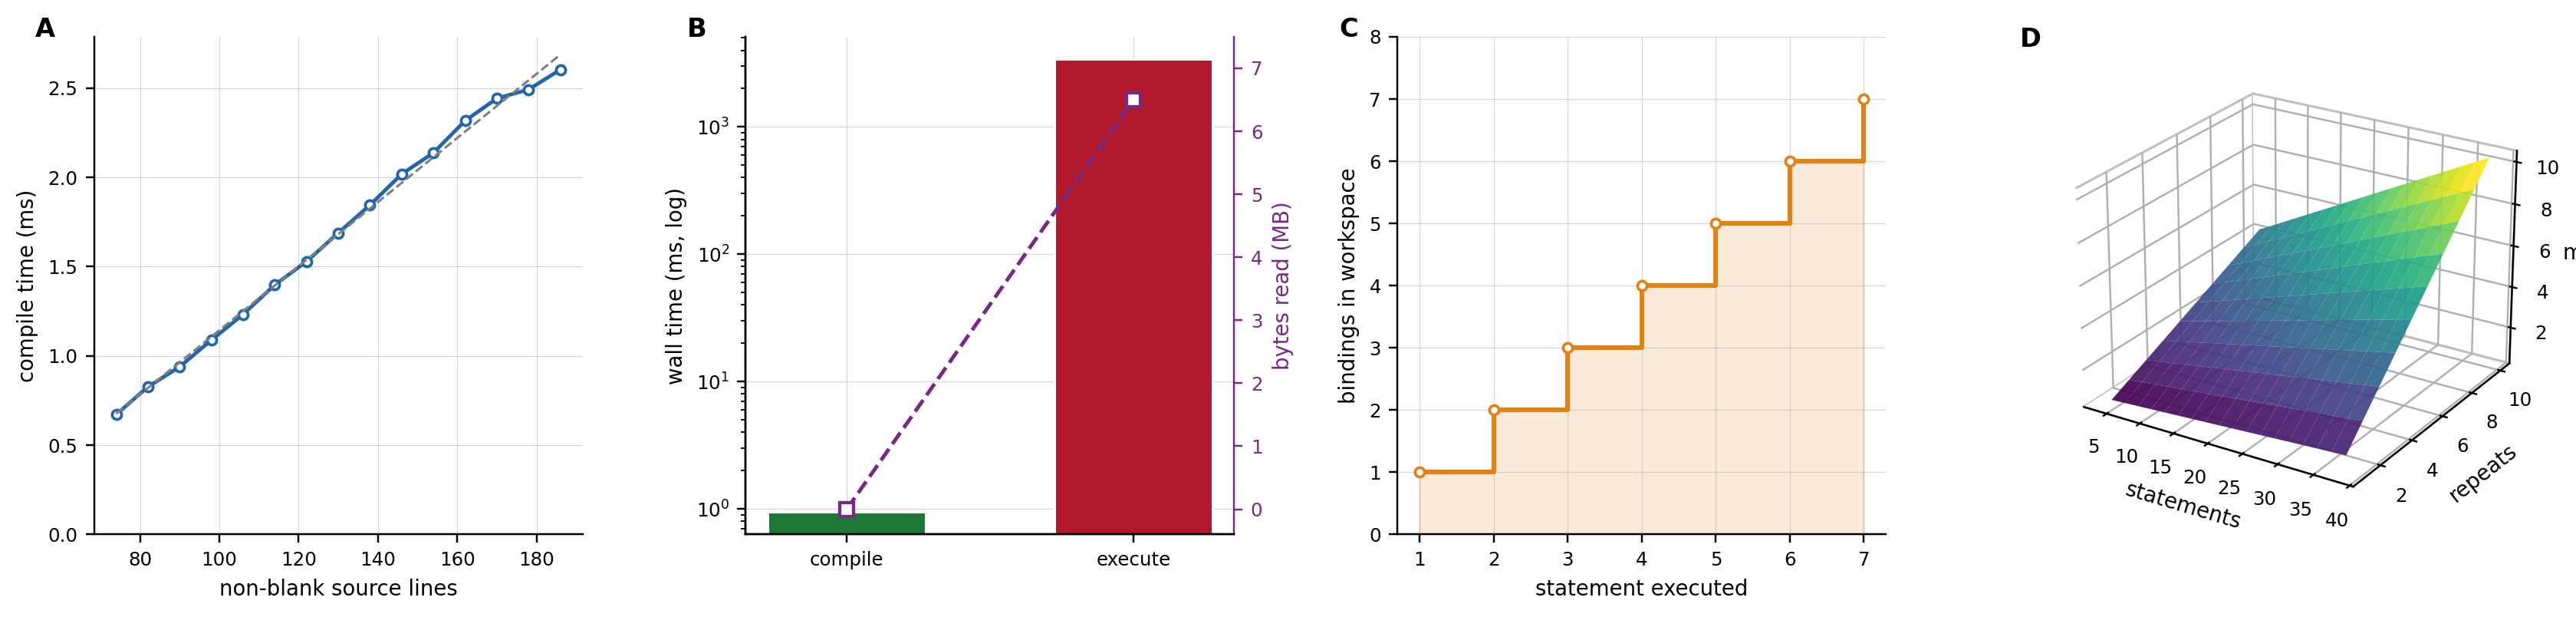
\includegraphics[width=\textwidth]{figures/panel1_compilation.png}
    \caption{\textbf{Two-stage compilation: checking cost, stage separation, and
    the append-only workspace.}
    (\textbf{A})~Compile-stage wall time against program length, measured as the
    minimum of forty repetitions at each size to suppress scheduler noise, over
    programs from $73$ to $187$ non-blank source lines constructed by appending
    replicate phases to the experiment program. The relation is linear (dashed
    fit), rising from $0.6$ to $2.5$~ms: parsing and structural checking scale
    with source length and with nothing else, which is what
    \Cref{thm:stage-separation} requires, since no clause of
    \Cref{def:structural} consults the environment or any operation denotation.
    (\textbf{B})~Cost of the two stages for the same program, wall time on a
    logarithmic axis (bars, left) against bytes read (squares, right). The
    compile stage takes $0.95$~ms and reads $0$~bytes; the execute stage takes
    $3.4$~s and reads $6.5$~MB. The ratio of approximately $1{:}3500$ in time,
    with a strict zero in I/O, is the observable content of
    \Cref{cor:effect-free}: a program that would read a reference library can be
    checked without reading it.
    (\textbf{C})~Workspace size after each executed statement of the experiment
    program. The trace is a monotone staircase reaching seven bindings and never
    decreasing, which is \Cref{thm:monotone}: no executed statement removes a
    binding, so the workspace at the end of a run is an append-only record of
    what the run produced.
    (\textbf{D})~Three-dimensional surface of compile time over the number of
    statements and the number of repeated compilations, extrapolated from the
    fitted slope of panel~A. The surface is planar in both arguments: checking
    cost is separable, with no interaction term, so repeated checking during
    editing carries no growing penalty.}
    \label{fig:ss-panel-01}
\end{figure*}

% ---------------------------------------------------------------------
%  Panel 2 - The coordinate space
% ---------------------------------------------------------------------
\begin{figure*}[!htbp]
    \centering
    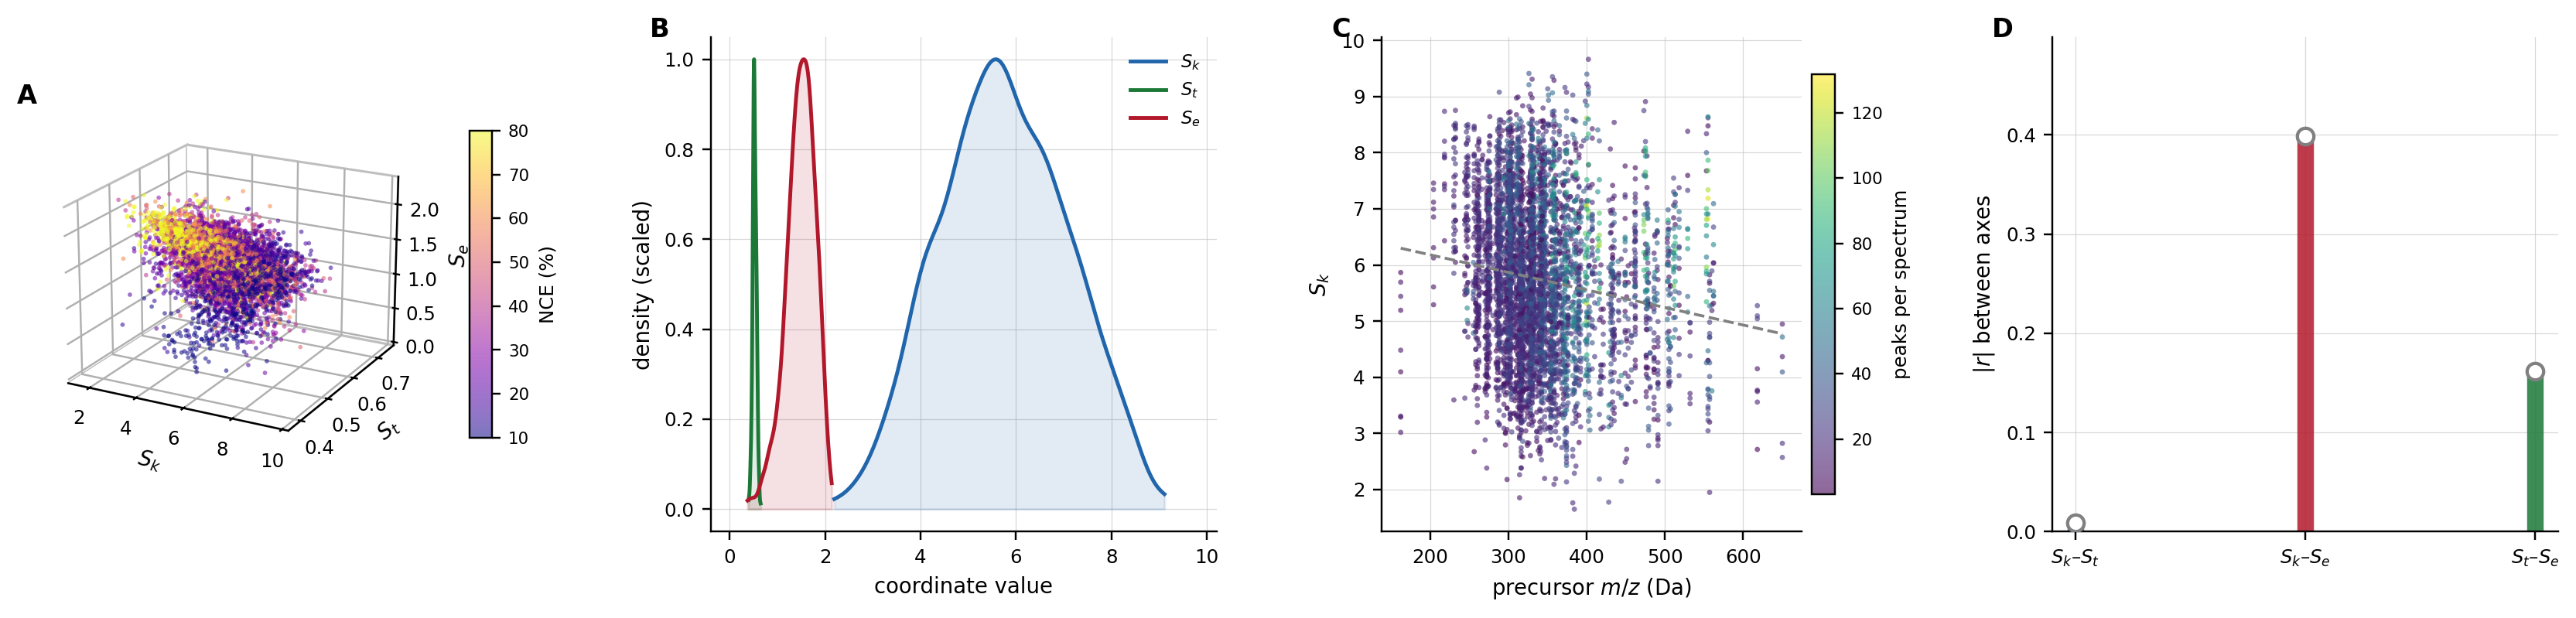
\includegraphics[width=\textwidth]{figures/panel2_coordinate_space.png}
    \caption{\textbf{Occupancy of the coordinate space over $5{,}298$ transformed
    spectra, and the structure of its three axes.}
    (\textbf{A})~Three-dimensional scatter of all admitted spectra in
    $(S_k, S_t, S_e)$, each point one spectrum, coloured by normalised collision
    energy from $10\%$ (dark) to $80\%$ (bright). The cloud is not homogeneous in
    colour: high-energy spectra occupy the upper-$S_e$, lower-$S_k$ region and
    low-energy spectra the opposite corner, so collision energy is already
    visible as a systematic direction through the space before any statistic is
    computed. This is the observation the remaining panels quantify.
    (\textbf{B})~Marginal densities of the three coordinates, each scaled to unit
    maximum. The axes occupy disjoint ranges and differ in spread by two orders
    of magnitude: $S_k$ has mean $5.74$ and standard deviation $1.34$, $S_e$ mean
    $1.48$ and deviation $0.31$, and $S_t$ mean $0.520$ and deviation $0.041$.
    An unweighted Euclidean distance over the three is therefore dominated by
    $S_k$, which \Cref{fig:ss-panel-04}(B) confirms.
    (\textbf{C})~Knowledge coordinate against precursor $m/z$, coloured by the
    number of peaks in the spectrum, with a least-squares fit. The relation is
    weak ($r = -0.147$, slope $-0.0031$ per dalton) while the colour gradient is
    strong and runs vertically: $S_k$ is governed by peak count rather than by
    precursor mass, which follows from \Cref{eq:sk}, whose leading term is the
    Shannon self-information of the normalised intensities.
    (\textbf{D})~Absolute Pearson correlation between each pair of axes. The
    $S_k$--$S_t$ pair is effectively uncorrelated ($0.009$) and $S_t$--$S_e$
    weakly so ($0.162$), but $S_k$--$S_e$ reaches $0.399$: two of the three axes
    share a substantial component, so the coordinate triple carries fewer than
    three independent degrees of freedom.}
    \label{fig:ss-panel-02}
\end{figure*}

% ---------------------------------------------------------------------
%  Panel 3 - Collision-energy dependence
% ---------------------------------------------------------------------
\begin{figure*}[!htbp]
    \centering
    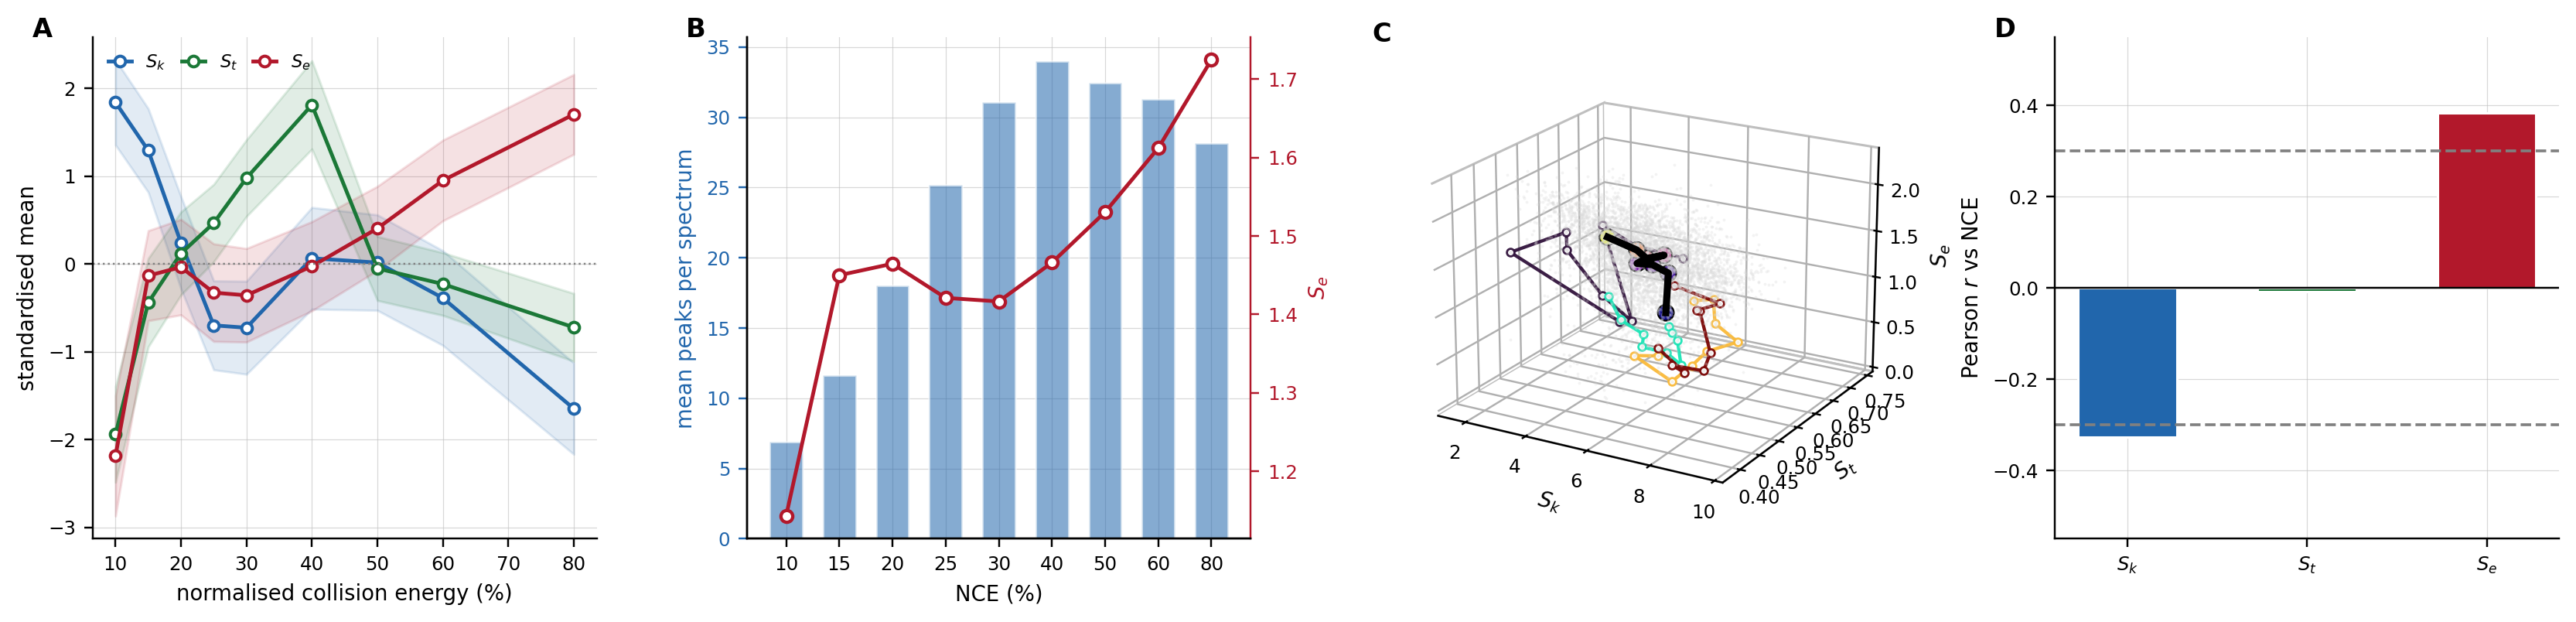
\includegraphics[width=\textwidth]{figures/panel3_nce_dependence.png}
    \caption{\textbf{The coordinates track collision energy, and the mechanism by
    which they do.}
    (\textbf{A})~Mean coordinate at each of the nine collision-energy levels,
    standardised per axis so the three overlay, with shaded bands at a fixed
    fraction of the within-level dispersion. $S_k$ falls from $6.97$ to $4.74$
    across the range and $S_e$ rises from $1.14$ to $1.73$, in opposite
    directions and monotonically over most of the range, while $S_t$ is flat.
    Collision energy is an experimental setting, not a property of the analyte;
    a coordinate that moves with it is reporting the setting.
    (\textbf{B})~Mean peaks per spectrum against collision energy (bars, left)
    with the mean evolution coordinate overlaid (line, right). Peak count rises
    from $6.9$ at $10\%$ to a maximum of $34.0$ at $40\%$ before falling to
    $28.1$ at $80\%$, and $S_e$ tracks it. This is the mechanism: \Cref{eq:se}
    is the Shannon entropy of the local intensity distribution, and adding
    fragments of comparable intensity raises that entropy directly. The
    correlation in panel~D is therefore not an artefact of the implementation
    but a consequence of what the definition computes.
    (\textbf{C})~Three-dimensional view of the same effect. The grey cloud is all
    spectra; four coloured paths follow individual analytes from low to high
    collision energy; the heavy black path joins the global centroid at each
    energy level, with markers coloured by that level. The centroid traverses a
    substantial fraction of the occupied region, so the drift is systematic
    across the library rather than confined to particular analytes.
    (\textbf{D})~Pearson correlation of each axis with collision energy against
    the threshold of $\lvert r\rvert < 0.3$ declared in the program (dashed
    lines). $S_t$ satisfies it at $-0.009$; $S_k$ fails at $-0.327$ and $S_e$
    fails at $+0.383$. Two of the three axes are outside the bound the
    experiment set for itself before it was run.}
    \label{fig:ss-panel-03}
\end{figure*}

% ---------------------------------------------------------------------
%  Panel 4 - Separation and the negative control
% ---------------------------------------------------------------------
\begin{figure*}[!htbp]
    \centering
    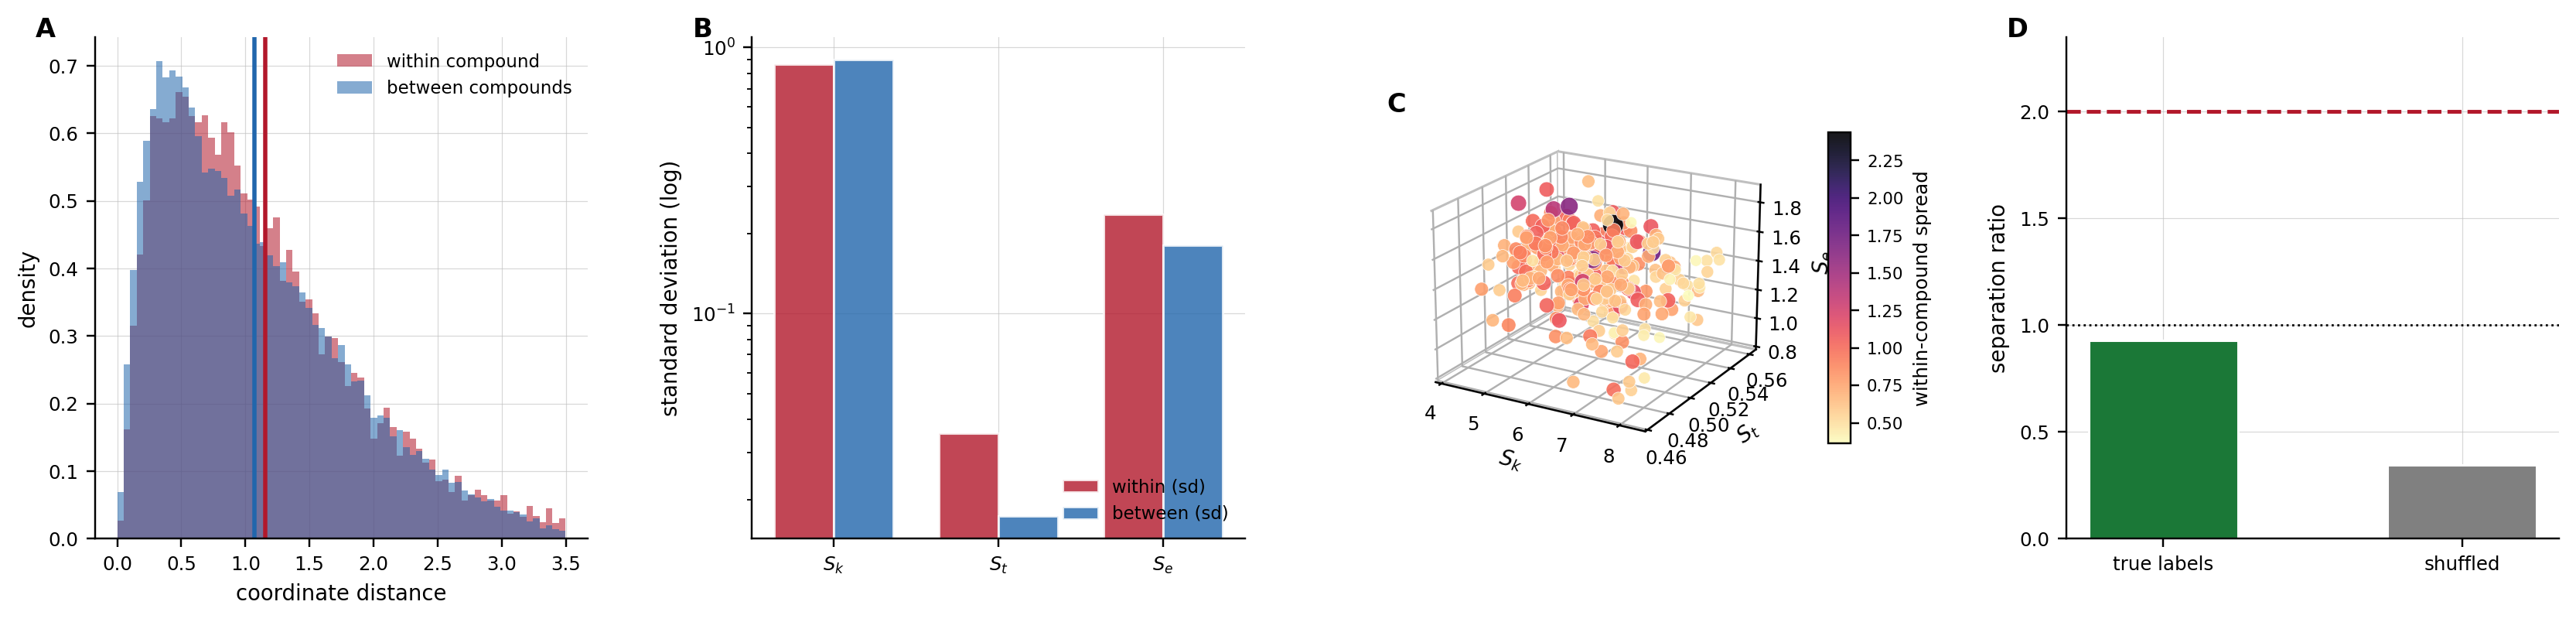
\includegraphics[width=\textwidth]{figures/panel4_separation.png}
    \caption{\textbf{Within-analyte and between-analyte coordinate spread over the
    $313$ analytes measured at all nine collision energies, with the label-shuffle
    control.}
    (\textbf{A})~Distributions of coordinate distance for the $11{,}268$ pairs of
    spectra of the same analyte at different collision energies (within) and the
    $48{,}828$ pairs of analyte centroids (between), with means marked. The two
    distributions are almost coincident, and the within-analyte mean of $1.155$
    slightly \emph{exceeds} the between-analyte mean of $1.074$. Changing the
    collision energy at fixed analyte moves a spectrum as far through the
    coordinate space as changing the analyte does; this single overlap is the
    experiment's result.
    (\textbf{B})~Per-axis standard deviations on a logarithmic scale, within
    analyte against between analytes. Only $S_k$ has between-analyte spread
    exceeding within-analyte spread, and then only marginally
    ($0.899$ against $0.865$, ratio $1.04$); $S_e$ gives $0.76$ and $S_t$ gives
    $0.49$. No axis discriminates analytes on its own, and the two orders of
    magnitude separating the $S_k$ and $S_t$ scales explain why the joint
    distance in panel~A is set almost entirely by $S_k$.
    (\textbf{C})~Three-dimensional scatter of the $313$ analyte centroids,
    coloured and sized by the mean distance from each analyte's spectra to its
    own centroid (range $0.36$ to $2.44$, median $0.73$). Centroid spacing and
    within-analyte spread are of the same order throughout the occupied region,
    which is the geometric statement of panel~A: the clusters are not separated
    by the scatter within them.
    (\textbf{D})~Separation ratio for true analyte labels and for labels permuted
    at a fixed seed, against the threshold of $2.0$ declared in the program
    (dashed) and the value $1.0$ at which grouping carries no information
    (dotted). The true ratio is $0.930$ and the shuffled ratio $0.347$. The
    control behaves as a control must: the statistic distinguishes real grouping
    from random grouping by a factor of $2.7$, so the apparatus discriminates
    and the failure to reach the threshold is a property of the transformation
    rather than of the measurement.}
    \label{fig:ss-panel-04}
\end{figure*}

% ---------------------------------------------------------------------
%  Panel 5 - The comparison method
% ---------------------------------------------------------------------
\begin{figure*}[!htbp]
    \centering
    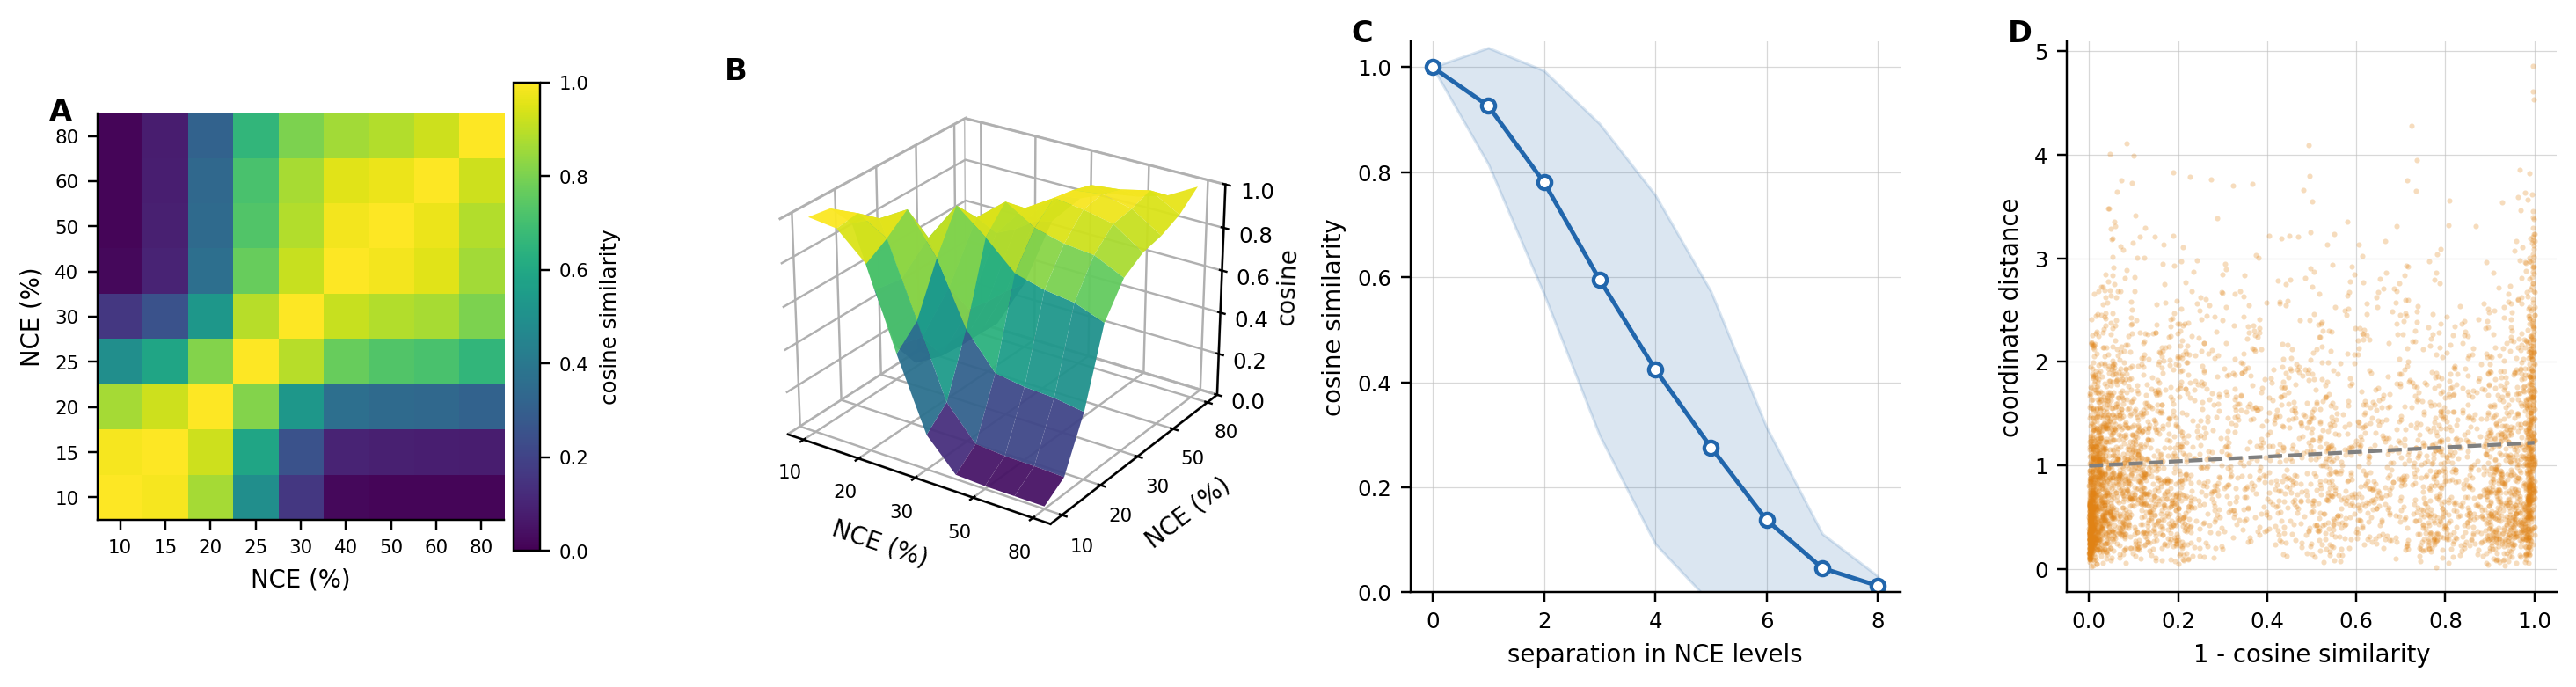
\includegraphics[width=\textwidth]{figures/panel5_baseline.png}
    \caption{\textbf{The declared comparison method: cosine similarity of raw peak
    lists across collision energy, over $5{,}400$ spectrum pairs from $120$
    analytes.}
    (\textbf{A})~Mean cosine similarity between every ordered pair of collision
    energy levels, matched within $0.01$~Da and averaged across analytes. The
    matrix is bright along and adjacent to the diagonal and dark at the corners,
    falling to $0.012$ between the $10\%$ and $80\%$ extremes. Raw spectra are
    stable under small changes in collision energy and unrecognisable under large
    ones, which is the established behaviour this method is known for.
    (\textbf{B})~The same matrix as a surface. The ridge along the diagonal is
    the region in which spectral matching is reliable; the two low corners are
    where it is not. The comparison method's competence is thus confined to a
    band, and the coordinate transformation was proposed to remove that
    restriction.
    (\textbf{C})~Mean similarity against separation in collision-energy levels,
    with a one-standard-deviation band. Similarity decays from $1.000$ at zero
    separation to $0.926$ at one level and $0.012$ at eight. The value at one
    level of separation is the relevant comparison: where the criterion required
    the coordinates to be stable under a change of collision energy, the
    incumbent method is stable to within $7\%$.
    (\textbf{D})~Coordinate distance against spectral dissimilarity for the same
    pairs, with a least-squares fit. The relation is positive but shallow and
    the scatter is wide: pairs whose raw spectra are nearly identical
    ($1 - \cos \approx 0$) span coordinate distances from $0$ to above $3$, and
    pairs whose spectra are entirely dissimilar span the same range. The
    coordinate distance is therefore not a monotone recoding of spectral
    similarity; it is a different quantity, and on this evidence a noisier one.}
    \label{fig:ss-panel-05}
\end{figure*}

% ---------------------------------------------------------------------
%  Panel 6 - Parameter dependence
% ---------------------------------------------------------------------
\begin{figure*}[!htbp]
    \centering
    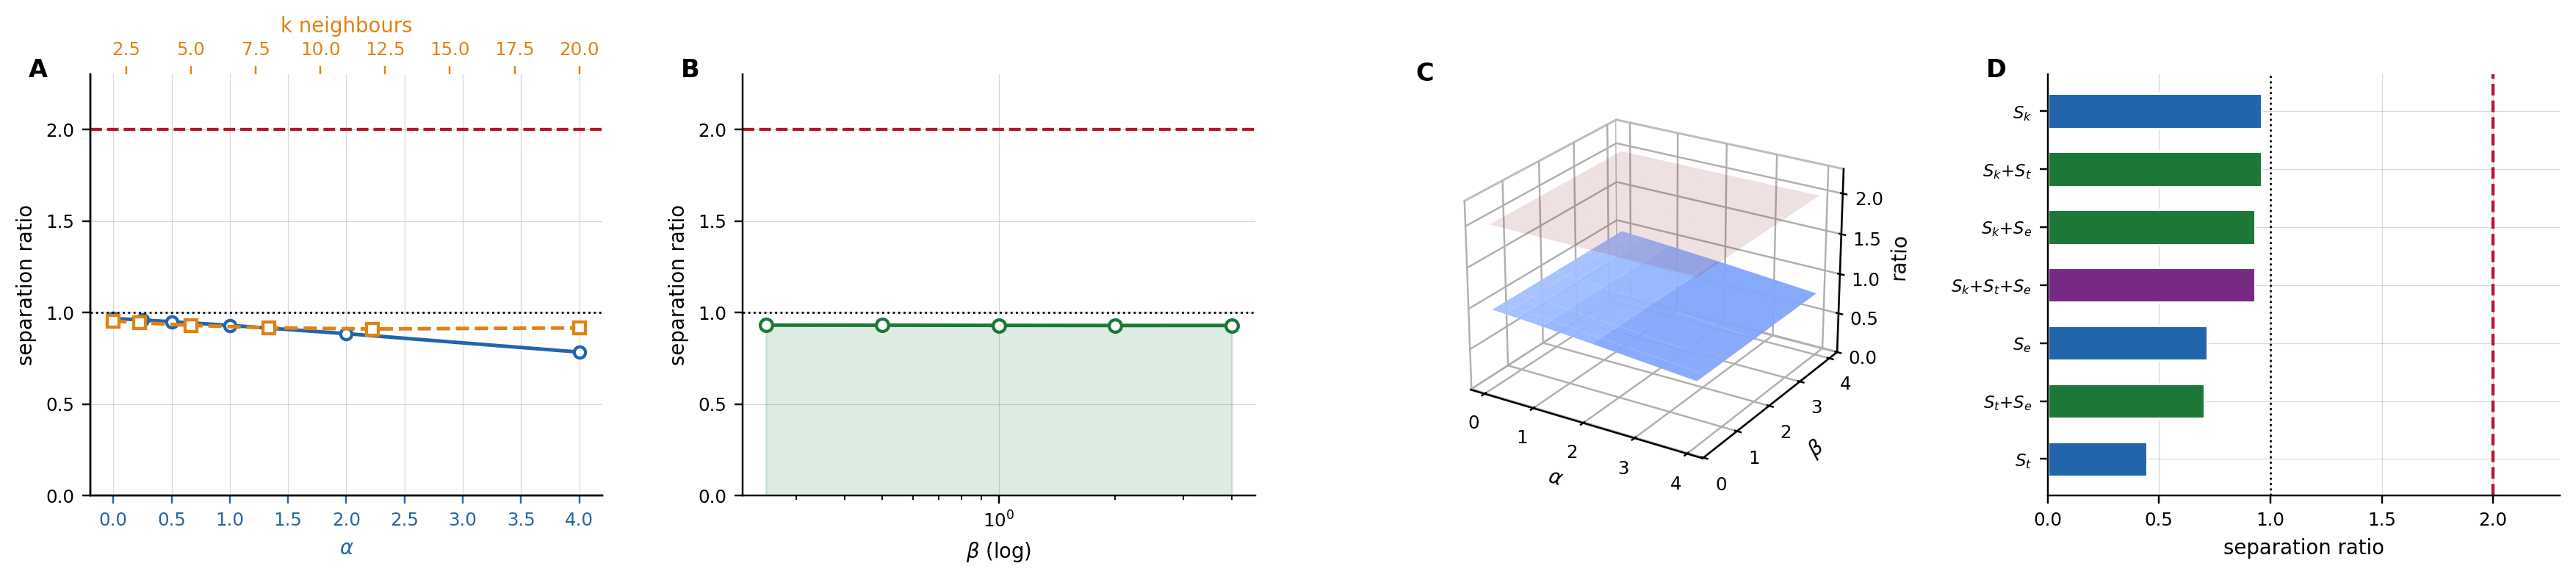
\includegraphics[width=\textwidth]{figures/panel6_parameters.png}
    \caption{\textbf{The outcome does not depend on the declared parameter values:
    forty settings and seven axis subsets, none reaching the threshold.}
    (\textbf{A})~Separation ratio against the mass weight $\alpha$ (circles,
    lower axis) and against the neighbourhood size $k$ (squares, upper axis),
    each varied with the others held at the declared values. The ratio falls
    monotonically in $\alpha$, from $0.968$ at $\alpha = 0$ to $0.784$ at
    $\alpha = 4$: the mass term of \Cref{eq:sk} separates spectra without
    separating analytes, so weighting it more heavily makes the statistic worse.
    Dependence on $k$ is weak across an order of magnitude
    ($0.954$ at $k=2$ to $0.916$ at $k=20$).
    (\textbf{B})~Separation ratio against the temporal weight $\beta$ on a
    logarithmic axis. The curve is flat to within $0.002$ across a sixteen-fold
    range, which follows from panel~B of \Cref{fig:ss-panel-04}: $S_t$ carries a
    spread two orders of magnitude below $S_k$, so reweighting it cannot move a
    joint Euclidean distance.
    (\textbf{C})~Three-dimensional surface of the separation ratio over
    $(\alpha, \beta)$ at fixed $k = 5$, with the declared threshold of $2.0$ drawn
    as a translucent plane. The surface is everywhere below the plane and
    everywhere below unity. The gap is not a near miss that a better parameter
    choice would close.
    (\textbf{D})~Separation ratio for each of the seven non-empty subsets of the
    three axes, ordered by value. The best is $S_k$ alone at $0.962$, marginally
    above the full triple at $0.930$; the worst is $S_t$ alone at $0.448$.
    Adding axes does not help and dropping them does not either, so the shortfall
    is not attributable to one axis contaminating the others. A grid search
    establishes no impossibility, and this one does not claim to; what it
    establishes is that the values declared in the program were not unlucky.}
    \label{fig:ss-panel-06}
\end{figure*}
